\documentclass[fleqn,10pt]{wlscirep}
\usepackage[utf8]{inputenc}
\usepackage[T1]{fontenc}
\usepackage{bm}
\title{CTSR Autonomous Fault detection with Neural Network}

\author[1,*]{Yong Dou(yd2373)}

\affil[1]{Columbia University, Department of Chemical Engineering ,New York, NY}

\affil[*]{e-mail:yd2373@columbia.edu}


\begin{abstract}

\end{abstract}
\begin{document}

\flushbottom
\maketitle

\thispagestyle{empty}

\noindent \textbf{Key points:} Please suggest $\sim 5$ key points, which should be single-sentence bullet points that summarize the article and remind readers of the take-home messages. An example of key points can be found at \url{https://www.nature.com/articles/s42254-018-0001-7#Abs3}

\noindent \textbf{Website summary:} Please suggest an $\sim 40$ word summary for the website.Please begin with a general sentence setting the background, then outline the topics discussed in the article. You can find example summaries at \url{https://www.nature.com/natrevphys/reviews}

\section*{Section headings max 38 characters for Reviews and 32 for Perspectives, with no punctuation beside commas}
\textit{Nature Reviews Physics} welcomes submissions in \LaTeX. For  peer-review purposes please just submit a .pdf file via our manuscript tracking system \url{https://mts-natrevphys.nature.com/}. Following peer-review and subsequent revisions we will ask for the .tex file and we will edit it using Overleaf. You will be able to follow the track changes and answer the editor's queries in Overleaf.

The published version will look very different from the accepted version of the manuscript. The figures will be redrawn by our art editors and the tables and boxes may be laid out  on one or two columns depending on different factors. This template is meant for peer-review and editing purposes and for this reason the layout does not reflect that of the published version. 

\subsection*{Subsection heading max 38 characters for Reviews and 32 for Perspectives}
There are three types of display items: figures (Fig. \ref{fig}), boxes (Box 1) and tables (Table \ref{tab}). Examples can be found at the end of the document.

If you cite a Book \cite{Book} please mention whether you are referring to the whole book or a certain chapter. You may also cite preprints\cite{arxiv} but where possible, please cite peer-reviewed literature.

\subsubsection*{Subsubsection heading max 80 characters (Reviews) or 70 characters (Perspectives)}
All equations should be numbered and all symbols should be defined. Example:
\begin{equation}\label{eq}
\hat{H} |\psi \rangle = E |\psi \rangle
\end{equation}
Here, $\psi$ is the wavefunction, $\hat{H}$ is the Hamiltonian and $E$ is the energy of the system. Vectors are typeset in bold italics, like this: $\bm{x}$.
\section*{Article types in Nature Reviews Physics}
\subsection*{Review}
A Review\cite{Review} is an authoritative, balanced survey of recent developments in a research field. Although Reviews should be recognized as scholarly by specialists in the field, they should be written with a view to informing non-specialist readers. Thus, Reviews should be presented using simple prose, avoiding excessive jargon and technical detail.

Reviews are approximately 5,000–-6,000 words long and typically include 7 display items (figures, tables or boxes). As a guideline, Reviews can contain up to 150 references, citations should be selective, and footnotes are not used. The scope of a Review should be broad enough that it is not dominated by the work of a single research institution and particularly not by the authors' own work.
\subsection*{Perspective}

A Perspective\cite{Perspective} is an opinionated review on an emerging field. They are more forward-looking and/or speculative than Reviews and may have a narrower scope. Despite being opinionated, they should remain balanced and are intended to stimulate discussion and new approaches.

Perspectives should typically be no more than 4,500 words long and include no more than 5 display items (figures, tables or boxes). Citations in Perspectives should be selective and as a guideline there should usually be no more than 100 references. 

\subsection*{Roadmap}

A Roadmap is a forward-looking outline of the scientific and technical challenges and opportunities in a certain field or for a specific big project. Roadmaps provide a sense of direction and set out the necessary steps that probably need to be achieved. They may also list a set of open questions. Roadmaps are authored by panels of experts.

Roadmaps are approximately 6,000–-8,000 words long and typically include 7 display items (figures, tables or boxes). As a guideline, they allow up to 100 references. 

\subsection*{Technical Review}

A Technical Review\cite{TR} surveys the current of state-of-the-art capabilities in a certain area. Technical Reviews provide accessible summaries of the state-of-the-art figures of merit for techniques, devices and/or materials; comparisons of different methods with an overview of their applicability; comparisons of scientific software codes for specific applications; guidelines for data analysis of specific datasets and in particular large data releases from big instruments.

Technical Reviews are approximately 5,000–-6,000 words long and typically include 8 display items and 150 references. 
\subsection*{Expert Recommendation}

Expert Recommendations are collective opinion pieces, authored by panels of specialists, that present the outcome of an analysis or discussion, and suggest a course of action, best scientific practices or methodological guidelines.

Expert Recommendations are typically 1,500–-2,000 words long and may include up to 4 display items and 50 references.

\bibliography{sample}

\noindent \textbf{For Reviews only, highlighted references (optional)} Please select 5–-10 key references and provide a single sentence for each, highlighting the significance of the work.

\section*{Acknowledgements (optional)}
The authors thank Erwin the Cat for useful discussions. Please edit as necessary.

\section*{Author contributions}
The authors contributed equally to all aspects of the article. Please edit as necessary. Note that the information must be the same as in our manuscript tracking system.

\section*{Competing interests}
The authors declare no competing interests. Please edit as necessary. Note that the information must be the same as in our manuscript tracking system.

\section*{Publisher’s note}
Springer Nature remains neutral with regard to jurisdictional claims in published maps and institutional affiliations.

\section*{Supplementary information (optional)}
If your article requires supplementary information, please include these files for peer-review. Please note that supplementary information will not be edited.

\newpage
\section*{Box 1 (Optional)}
This is a Box, which can contain a figure, and which should have no more than 300 words of text.

\begin{figure}[ht]
\centering
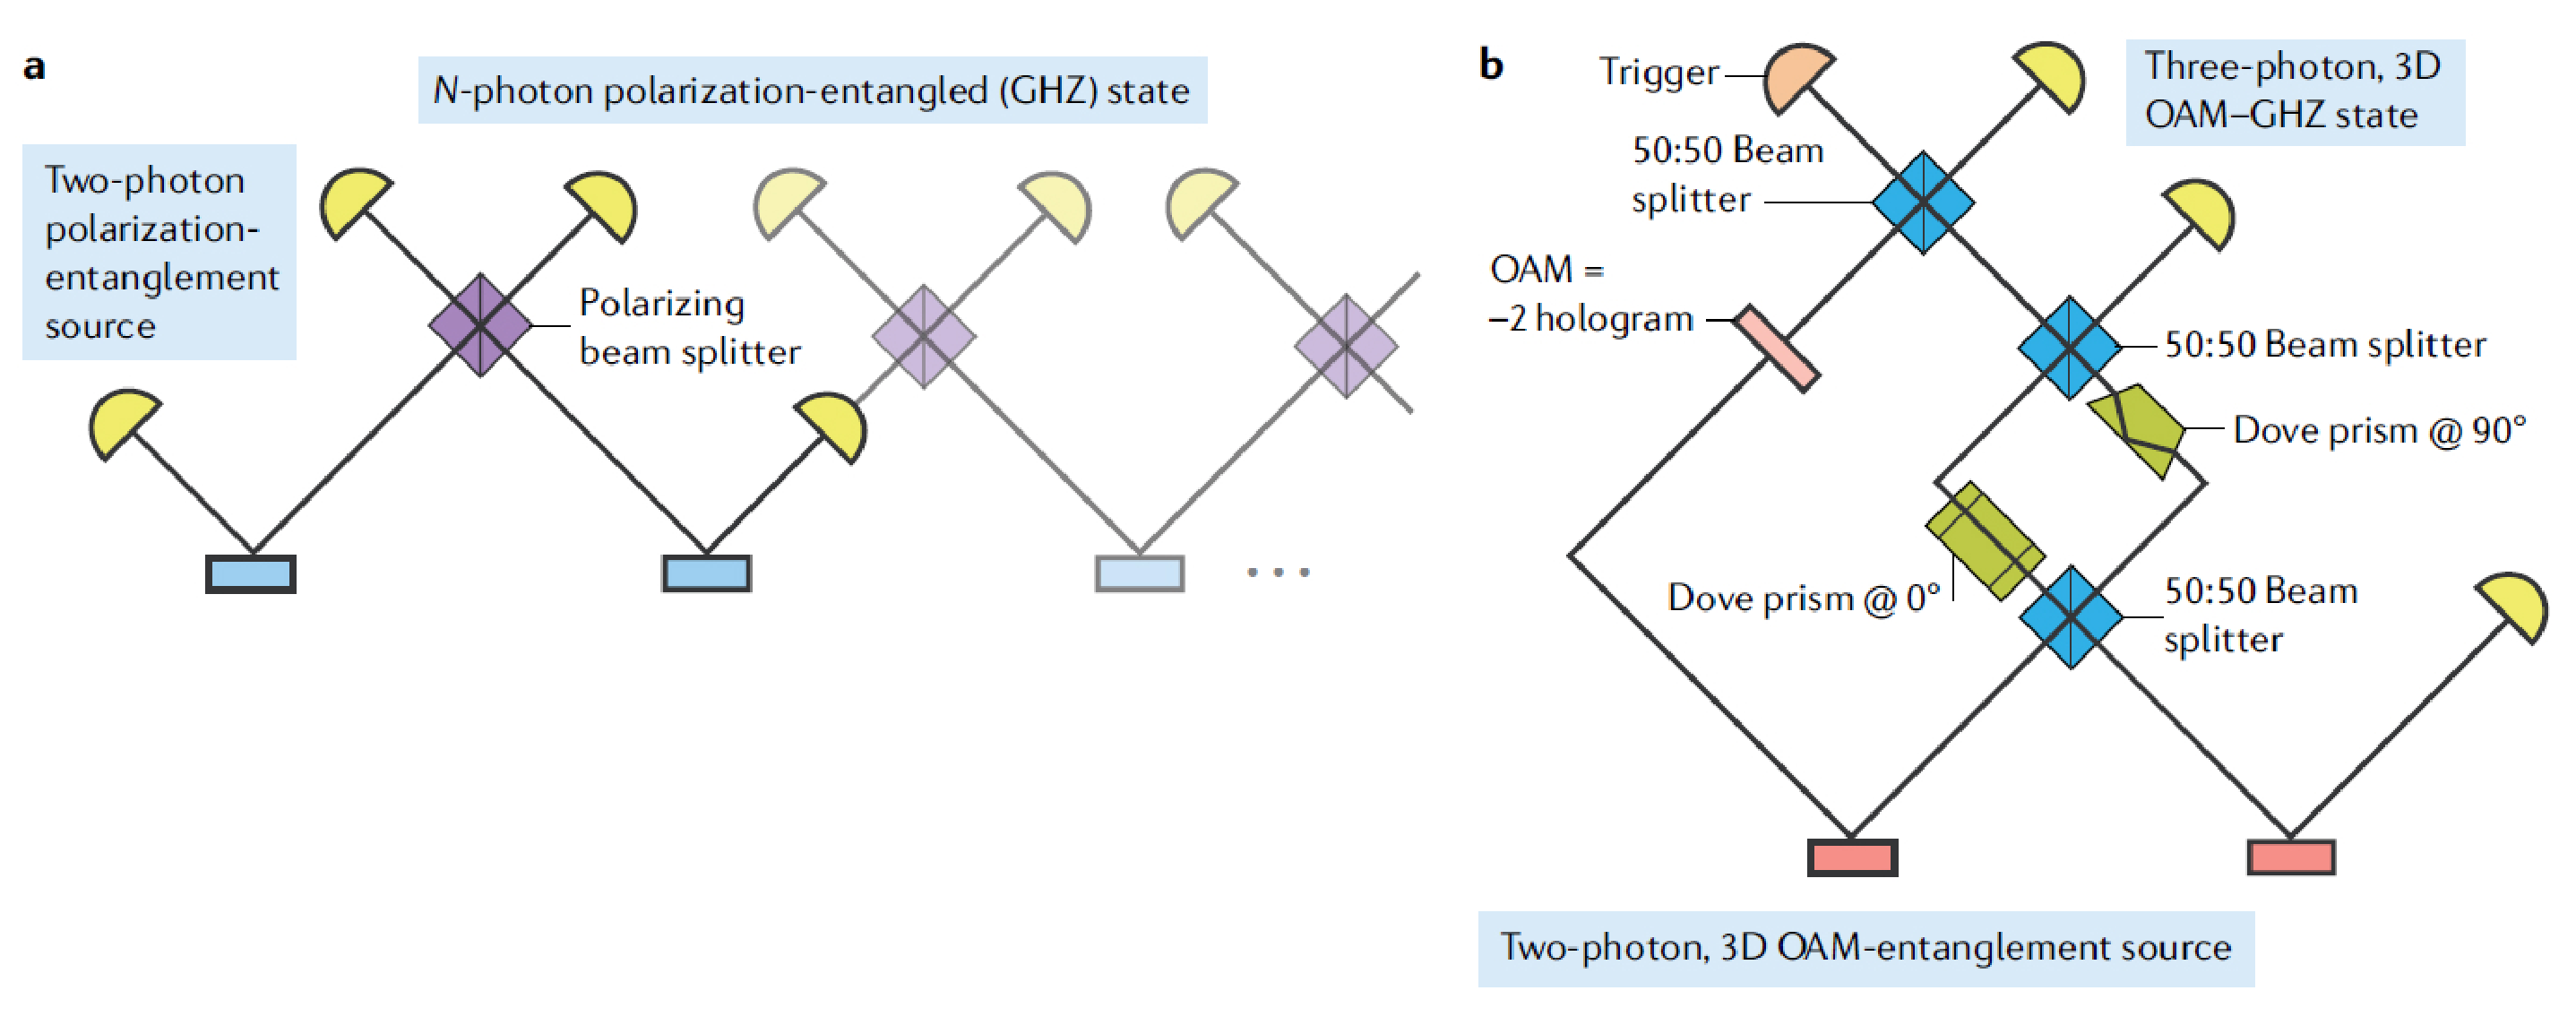
\includegraphics[width=\linewidth]{fig}
\caption{The figure caption should start with a title explaining the figure. Figures should be self-consistent so please redefine all acronyms and define all symbols. Example: GHZ, Greenberger–Horne–Zeilinger, OAM, orbital angular momentum. Please provide credit lines for panels reproduced from the literature. Example: Panels a and b are reproduced from Ref. \cite{TR}.}
\label{fig}
\end{figure}

\begin{table}[ht]
\centering
\begin{tabular}{|l|l|l|}
\hline
Particle & Mass & Charge \\
\hline
Electron & $9.10938356(11)\times10^{-31}$ kg & $-1e$ \\
\hline
Proton & $1.672621898(21)\times10^{-27}$ kg & $+1e$ \\
\hline
Neutron & $1.674927471(21)\times10^{-27}$ kg & $0$ \\
\hline
\end{tabular}
\caption{\label{tab}Tables have titles but no captions are allowed. However, all symbols and acronyms used in a table should be defined in a footnote. Example: Here $e$ is the elementary charge.}
\end{table}

\section*{Glossary terms (optional)}
It is possible  to include glossary terms to define some technical terms. For each glossary term, please provide a short (maximum 30 word) definition. Please list these in order of first appearance in the text. In the published version, they will appear in the margins of the document. 

Example: \\
\textbf{Lam\'e parameters:} A possible pair of parameters that characterize the Cauchy elasticity tensor in an isotropic homogeneous medium. The second Lam\'e parameter is identical to the shear modulus.



\end{document}